\documentclass{article}
\usepackage[utf8]{inputenc}

\usepackage{natbib}
\usepackage{amsthm}
\usepackage{amssymb}
\usepackage{float}
\usepackage{algorithm}
\usepackage{algpseudocode}
\usepackage{listings}

\usepackage{amsmath}%
\usepackage{MnSymbol}%
\usepackage{wasysym}%
\usepackage{graphicx}
\usepackage{csquotes}
\usepackage{geometry}
 \geometry{
 a4paper,
 total={170mm,257mm},
 left=30mm,
 right=30mm,
 top=20mm,
 }
\newcommand{\argmax}{\arg\!\max}
\newcommand*{\QEDA}{\hfill\ensuremath{\blacksquare}}%

\begin{document}
\begin{titlepage}
\begin{center}

\vspace*{10cm}
{\large Master 1 MoSIG}\\[0.5cm]

{\Huge \textbf{Algorithmic Problem Solving} }\\[0.5cm]
{\large APP3 Report}\\
Hole Drilling\\ 
Team:\\SACAD
\vfill

% Author and supervisor
\noindent
\begin{minipage}{0.4\textwidth}
   \centering Members:\\
   Andrey \textbf{SOSNIN}\\
   Majdeddine \textbf{ALHAFEZ}\\
   Antoine \textbf{COLOMBIER}\\
   Eman \textbf{AL-SHAOUR}\\
   Son Tung \textbf{DO}\\
\end{minipage}%

\vfill
% Bottom of the page
{Grenoble, 12 November, 2017}
\end{center}
\end{titlepage}
\clearpage

\section{Discussion on the current algorithm}


\subsection{Not an $\alpha$-approximation}
Let us assume that we have $N$ points to drill and they are arranged as shown in figure1 where the distance between two horizontal points equals $2N$ and the distance between two vertical points equals to $1$.

\begin{figure}[h]
\centering 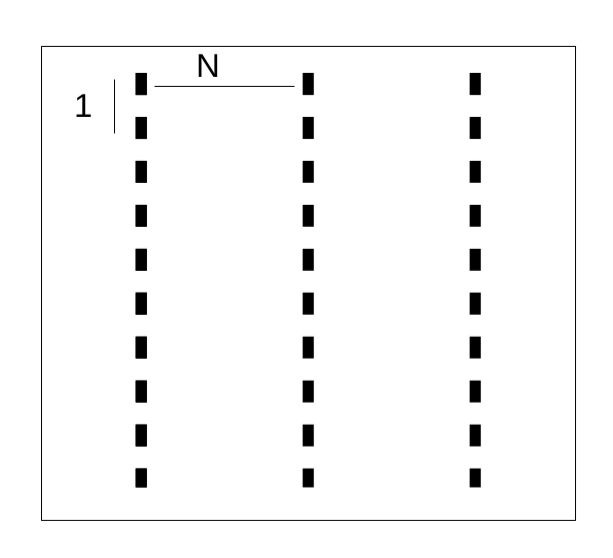
\includegraphics[width=0.3\linewidth]{F0.jpg}
\caption{circuit board}
\end{figure}

\begin{figure}[h]
\centering 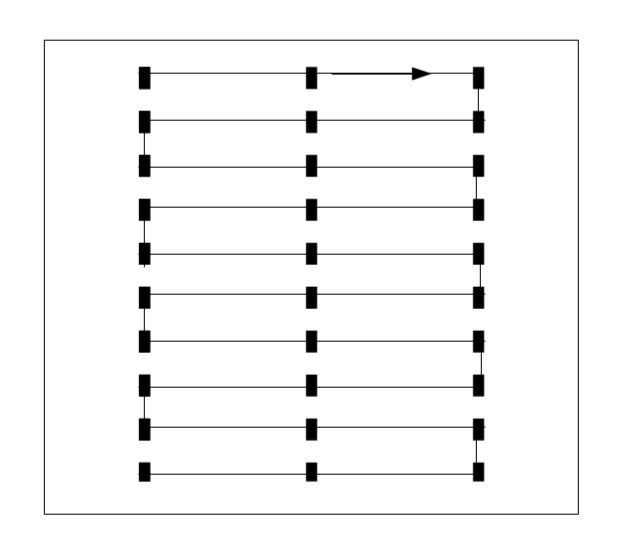
\includegraphics[width=0.3\linewidth]{F1.jpg}
\caption{behavior of the current algorithm}
\end{figure}

\begin{figure}[h]
\centering 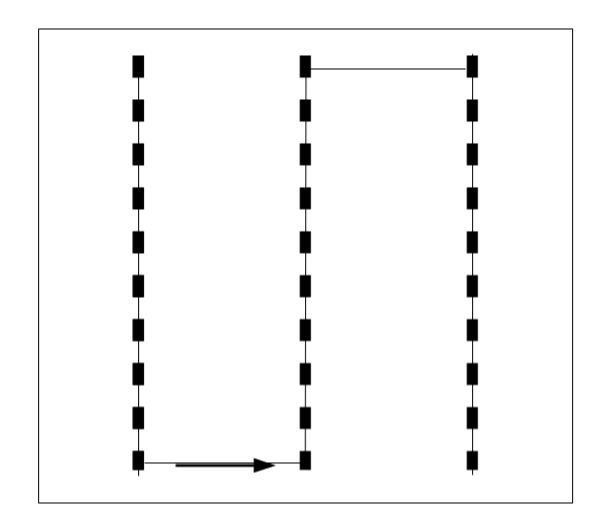
\includegraphics[width=0.3\linewidth]{F2.jpg}
\caption{behavior of the greedy algorithm}
\end{figure}

Figure 2 shows the behavior of the current algorithm (this is the best behavior based on the given description where after drilling all the points in a row, we drill the point just bellow the last drilled point). The total cost of the path is 
$C = O(N^{2})$

Figure 3 shows the behavior of what seems to be a better solution where we have $C' = O(N)$
The ratio is $O(N)$ and therefore such $\alpha$ doesn't exist and the current algorithm is not an $\alpha$-approximation.

\section{Greedy Approach}
\subsection{Propose an algorithm}
This greedy approach consists of going through the set of points picking up the point with the minimum distance to the current point.\\

In order to compute the algorithm using the notation of point, we have a data structure for point
\begin{lstlisting}
point {
	int x; /* x-coordinate */
	int y; /* y-coordinate */
}
\end{lstlisting}


\begin{algorithm}[H]
\caption{Greedy Approach}
\textbf{Input: }$A[N]$ array of N points to drill\\
\textbf{Output: } Array $A[N]$ with the order in which we drill the points
\begin{algorithmic} 
\For{\texttt{k from 0 to N}}
    \State $index \leftarrow -1$
    \State $min\_distance \leftarrow \infty $
    \For{\texttt{i from k+1 to N}}
        \State $distance \leftarrow find\_distance(A[k], A[i])$
        \If{$ distance < min\_distance$}
            \State $index = i$ 
            \State $min\_distance \leftarrow distance$
        \EndIf
    \EndFor
    \State $swap\_elements(k+1, index)$
\EndFor
\end{algorithmic}
\end{algorithm}
The function $find\_distance(p_{1}, p_{2})$ calculate the Euclidean distance between two points which is given by:
$distance = \sqrt{(x_{1}-x_{2}){^2} + (y_{1}+y_{2})}{^2} $ \\[0.3cm]
The complexity of this proposed algorithm is $O(N^{2})$. The essential of this algorithm is similar to a sorting problem which can be implemented with complexity of $O(N \times log(N))$, but we still need compute the distance that costs $O(N^{2})$ 
\subsection{Showing it is not optimal}
As we can see on figure4 bellow, the greedy solution is not optimal. Due to fact that the best choice in a local context might not be the best one for the final solution as we implement it in our greedy algorithm, we can then, admit that this solution is not solvable by a direct greedy solution.

\begin{figure}[h]
\centering 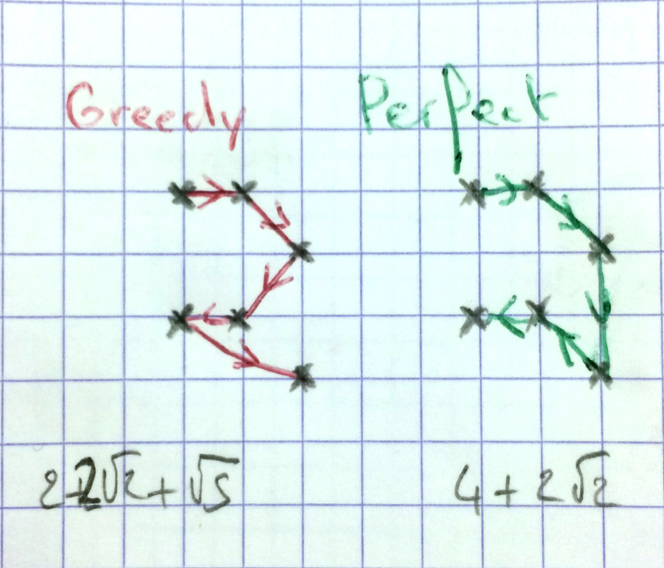
\includegraphics[width=0.5\linewidth]{not_optimal.png}
\caption{greedy vs optimal}
\end{figure}

\section{Minimum Spanning Tree - MST}

\subsection{Propose an algorithm}
In MST, we have nodes (the notation of point in our circuit board) and edges (represent the distance between 2 points in our circuit board).The idea of proposed algorithm based on the MST is to start with 1 node, we travel to the neighbors nodes. When we come to one neighbor node, we need explore its neighbors, except for the node we come from, until there is no neighbor in that node. At the node which have no neighbor but the previous node, we come back.

\begin{algorithm}[H]
\caption{Algorithm based on MST}
\textbf{Input: }MST for the point\\
\textbf{Output: }The $result\_array$ stores points in order that we need to move the drill
\begin{algorithmic} 
\Procedure{explore}{node, previous\_node} \Comment first call, we can have the previous\_node is null
\State $result\_array \leftarrow node$  \Comment add the current node to the result\_array
\While{\texttt{exist a neighbor except the previous node}}
    \State $explore(one neighbor, node)$
\EndWhile
\State $result\_array \leftarrow node$ \Comment add the current node to the result\_array again due to revisit
\EndProcedure
\end{algorithmic}
\end{algorithm}

The whole pseudo-code is included in file algo\_MST\_based.

\subsection{2-approximation proof}
We know that every spanning tree is more expensive than the weight of the MST, thus making a lower bound regarding the optimal solution :
$MST \leq C^{*}$  (1)\\
Our algorithm consider the MST of the holes, in the worst case, we go through every edge in MST twice.
$C = 2 \times MST$  (2)\\ 
From (1) and (2) we have $C \leq 2 \times C^{*}$.\\
We conclude that the algorithm is a 2-approximation.

\section{Correctness of Kruskal's algorithm}

We note by $w$ the weight function.

We want to show that Kruskal's algorithm returns the minimal spanning tree.

First, the result is clearly a spanning tree since it doesn't have any cycles, and it is connected (as otherwise we would have encounter an edge that connects two disconnected parts without creating a cycle since the initial graph is connected). Now we are going to prove that it is minimal. 
Let $K$ be the spanning tree produced by Kruskal's algorithm and $T$ be an arbitrary spanning tree. 
We are going to show that by gradually transforming $K$ into $T$ by adding and removing edges, we can only increase its weight (therefore we will have $w(T)\geq w(K)$).

First, note that $K$ and $T$ have the same number of edges ($|V|-1$) as they are both connected and acyclic. Suppose $T\neq K$. Let $e_{min}$ be the edge with the minimum weight in $T\backslash K$. 

Let $C = \{e_1,e_2,...,e_k,e_{min}\}$ be the elementary cycle created by adding $e_{min}$ to $K$. Let $e_j \in C \backslash T$ ($e_j$ exists since the $C$ is not contained in $T$, which is a tree). We have $w(e_j)\leq w(e_{min})$, since otherwise Kruskal would have chose $e_{min}$ over $e_j$. Consider $K' = (K\backslash \{e_j\})\cup\{e_{min}\}$. $K'$ is a spanning tree, but its weight is greater or equal to the weight of $K$ and $|K'\cap T| > |K \cap T|$. 

Repeating the described procedure a finite number of times on $K'$ in the place of $K$ etc will produce $T$. Thus $w(T)\geq w(K)$.

\end{document}
